% =====================================================================
% Informe del trabajo de señales — PSIB 2026Q2, Grupo 08
% Acoplamiento cardiopulmonar derivado del ECG como criterio de detección
% de apnea del sueño
%
% Compilar desde esta carpeta:   latexmk -pdf informe.tex
% (pdflatex + biber; en Overleaf funciona tal cual).
%
% Límite de la consigna: 8 páginas de cuerpo + 4 de anexo. Entrega: 10/11, 17:00.
% En modo borrador la portada dice dónde termina el cuerpo y el anexo.
% Los textos en rojo (\pendiente) son lo que falta escribir y los "?" rojos
% (\falta) son números que salen de notebooks/99_test.ipynb. Antes de entregar,
% pasar a \borradorfalse y revisar que el log no tenga avisos "Pendiente".
%
% Fuentes de los números: docs/esquema_v3.md (secciones 4 y 5),
% docs/plan_test.md y los notebooks de cada etapa.
% =====================================================================
\documentclass[11pt,a4paper]{article}

% ---------- Modo ----------
\newif\ifborrador
\borradortrue    % \borradorfalse para la versión de entrega

% ---------- Paquetes ----------
\usepackage[T1]{fontenc}
\usepackage{newtxtext,newtxmath}          % Times, como el informe de imágenes
\usepackage[spanish,es-tabla,es-noindentfirst]{babel}
\usepackage{microtype}
\usepackage[margin=2.2cm]{geometry}
\usepackage{amsmath}
\usepackage{graphicx}
\usepackage{booktabs}
\usepackage{tabularx}
\usepackage{xcolor}
\usepackage[font=small,labelfont=bf]{caption}
\usepackage{subcaption}
\usepackage{enumitem}
\setlist{nosep, leftmargin=*}
\usepackage{tikz}
\usetikzlibrary{positioning, arrows.meta, babel}
\usepackage{csquotes}
\usepackage[backend=biber, style=authoryear, maxcitenames=2, maxbibnames=10,
            uniquelist=false, uniquename=init, giveninits=true, doi=true, url=false,
            isbn=false]{biblatex}
\addbibresource{referencias.bib}
\usepackage[hidelinks]{hyperref}   % siempre al final

\graphicspath{{figuras/}}

% ---------- Datos de la portada ----------
\newcommand{\titulo}{Trabajo de señales: acoplamiento cardiopulmonar derivado del ECG
                     como criterio de detección de apnea del sueño}
\newcommand{\materia}{16.63 - Procesamiento de Señales e Imágenes Biomédicas 2026Q2}
\newcommand{\fecha}{10 de noviembre de 2026}
\newcommand{\repo}{\url{https://github.com/afrateitba/TP-PSB-G8}}

% ---------- Comandos propios ----------
% Texto que falta escribir: rojo en borrador; en la entrega desaparece y deja un aviso en el log.
\newcommand{\pendiente}[1]{%
  \ifborrador\textcolor{red}{[#1]}%
  \else\PackageWarning{informe}{Pendiente sin resolver en la pagina \thepage}\fi}
% Número que falta (sale de test).
\newcommand{\falta}{\ifborrador\textcolor{red}{?}\else\PackageWarning{informe}{Falta un numero en la pagina \thepage}\fi}

% Intervalo de confianza: \ic{0,760}{0,916}
\newcommand{\ic}[2]{(#1 a #2)}

% =====================================================================
\begin{document}

% ---------- Portada (modelo: informe del trabajo de imágenes) ----------
\begin{titlepage}
  \centering
  \vspace*{0.4cm}
  
\includegraphics[width=0.62\textwidth]{logo_itba.png}\par
  \vspace{1.4cm}
  \rule{\linewidth}{0.5pt}\par
  \vspace{0.35cm}
  {\Large \titulo\par}
  \vspace{0.25cm}
  \rule{\linewidth}{0.5pt}\par
  \vspace{1.0cm}
  {\large\bfseries \materia\par}
  \vspace{1.0cm}
  {\large\bfseries Grupo 8\par}
  \vspace{0.15cm}
  {\large Augusto Frate -- 65013\\[0.1cm]
          Karolina Tenca -- 62751\\[0.1cm]
          Leah Weizman -- 69550\par}
  \vspace{1.0cm}
  {\large\bfseries Profesores\par}
  \vspace{0.15cm}
  {\large Roberto Sebastian Tomas\\[0.1cm]
          Francisco Tassara\\[0.1cm]
          Lucila Capurro\\[0.1cm]
          Victoria Reppucci\par}
  \vfill
  {\fecha\par}
  \ifborrador
    \vspace{0.4cm}
    {\small\color{red}Borrador. El cuerpo termina en la página \pageref{fin-cuerpo} (límite: 8);
    el anexo va de la página \pageref{inicio-anexo} a la \pageref{fin-anexo} (límite: 4).\par}
  \fi
\end{titlepage}

% =====================================================================
\section{Introducción}
\label{sec:intro}

\subsection{Marco teórico}
\label{sec:marco}

La apnea del sueño se caracteriza por episodios repetidos de interrupción
o reducción de la respiración durante el descanso. En la apnea obstructiva,
estos episodios se producen por el cierre total o parcial de la vía aérea
superior, aunque se mantiene el esfuerzo respiratorio. Para su diagnóstico
se utiliza la polisomnografía, que registra distintas señales fisiológicas
y permite identificar los eventos respiratorios y su relación con el sueño.
A partir de este estudio se calcula el índice de apnea-hipopnea (AHI), que
expresa la cantidad de apneas e hipopneas por hora de sueño
\parencite{kapur2017}.

El interés por detectar apnea a partir del ECG surge porque los episodios
respiratorios también pueden manifestarse en la actividad cardíaca.
Durante la apnea pueden aparecer variaciones cíclicas de la frecuencia
cardíaca, que se observan en los intervalos entre picos R consecutivos.
Estos intervalos forman la serie RR y permiten estudiar la variabilidad
de la frecuencia cardíaca (HRV), tanto en el tiempo como en la frecuencia
\parencite{taskforce1996,penzel2002}. A su vez, la respiración modifica la
posición del corazón respecto de los electrodos y la impedancia del tórax,
lo que genera cambios en la amplitud y el área del complejo QRS. A partir
de estas variaciones puede obtenerse una señal de respiración derivada
del ECG, denominada EDR \parencite{moody1985}. De esta manera, un mismo
registro permite obtener información sobre las variaciones cardíacas y
respiratorias.

La relación entre ambas señales puede estudiarse mediante el análisis
del acoplamiento cardiopulmonar. Para ello se utilizan medidas como la
potencia cruzada, que permite identificar componentes compartidas en
distintas frecuencias, y la coherencia, que cuantifica su asociación
lineal normalizada. \textcite{thomas2005} utilizaron este enfoque para
caracterizar distintos regímenes de acoplamiento durante el sueño.
Este antecedente permite plantear que las oscilaciones lentas compartidas
entre RR y EDR podrían aportar información para detectar apnea, además
de la que ofrece el análisis de la variabilidad cardíaca por separado.

\subsection{Estado del arte}
\label{sec:estado}

La detección de apnea a partir del ECG fue el objetivo del
PhysioNet/Computers in Cardiology Challenge 2000, para el cual se
desarrolló la base Apnea-ECG utilizada en este trabajo. En una comparación
de trece algoritmos participantes, \textcite{penzel2002} encontraron que
los mejores resultados se obtenían al analizar características
espectrales de los intervalos cardíacos y de las variaciones del ECG
asociadas con la respiración. Dos de los métodos superaron el 90~\%
de exactitud en la clasificación por minuto, lo que mostró el potencial
de estas señales para identificar episodios de apnea.

En esta misma línea, \textcite{dechazal2003} combinaron características
de los intervalos entre latidos y del EDR mediante clasificadores
discriminantes lineales y cuadráticos, y alcanzaron una exactitud por
minuto superior al 90~\% en un conjunto independiente. Por su parte,
el trabajo de \textcite{thomas2005} permitió estudiar la relación entre
ambas señales desde el acoplamiento cardiopulmonar y vincularla con
la estabilidad del sueño. Estos antecedentes motivan el uso conjunto
de RR y EDR, aunque sus resultados corresponden a métodos y condiciones
de evaluación que deben considerarse al compararlos con otras propuestas.

A partir de estos antecedentes, en este trabajo se estudia una feature
conjunta RR--EDR basada en la potencia cruzada en la banda lenta asociada
al ciclo de apnea. Se busca determinar si esta información permite
mejorar la detección por minuto respecto de una feature basada únicamente
en la variabilidad cardíaca, utilizando un punto de corte estadístico
y sin aprendizaje automático. Las características y el umbral se eligen
con los registros de desarrollo, mientras que la evaluación final se
realiza sobre sujetos reservados para test. La propuesta se plantea como
un análisis de la información contenida en el ECG y no como un reemplazo
de la polisomnografía.

\subsection{Objetivos e hipótesis}
\label{sec:objetivos}

El objetivo es detectar la apnea del sueño minuto a minuto a partir del ECG, con un punto de
corte estadístico y sin aprendizaje automático. Se plantean dos hipótesis:

\begin{description}[leftmargin=0pt, labelindent=0pt, itemindent=!]
  \item[H1.] Durante la apnea aparece un acoplamiento lento entre la serie RR y el EDR, en la
    banda del ciclo de apnea (0,01 a 0,1~Hz), dentro de cada sujeto. El acoplamiento
    respiratorio (0,15 a 0,4~Hz) no desaparece.
  \item[H2.] La feature conjunta RR--EDR (F) detecta la apnea mejor que la mejor feature de
    variabilidad cardíaca, que usa solo el RR.
\end{description}

% =====================================================================
\section{Materiales y métodos}
\label{sec:metodos}

\subsection{Base de datos y adquisición}
\label{sec:base}

Se usó la Apnea-ECG Database de PhysioNet \parencite{penzel2000,goldberger2000}: 70
registros nocturnos de ECG de una derivación, muestreados a 100~Hz con 12 bits, con una
etiqueta de apnea o normal por minuto asignada por un experto a partir de la polisomnografía.
Ocho registros incluyen la respiración, que se usó solo para validar. Como a 100~Hz el pico R
queda cuantizado a 10~ms, se lo ubica a $\pm 30$~ms de cada marca de QRS de la base, según la
polaridad del registro, y se refina con una parábola de 3 puntos; el refinamiento se verificó
con una prueba de dos fases a 50~Hz.

Tres pares de registros resultaron ser la misma grabación (c05/c06, x22/x35 y x33/x34); se
excluyó uno de cada par y quedaron 67. Como la base no identifica a las personas, se agruparon
los registros con igual perfil (edad, sexo, altura y peso), lo que dio 29 sujetos. La
partición 70/30 se sorteó por sujeto con semilla 2026 (tabla~\ref{tab:particion}), con cuotas
exactas por categoría, una diferencia de 2 puntos o menos en la fracción de minutos con apnea
y los registros con respiración en desarrollo.

\begin{table}[htbp]
  \centering
  \caption{Partición por sujeto. Categoría A: 100 minutos de apnea o más; B: de 5 a 99;
           C: menos de 5.}
  \label{tab:particion}
  \begin{tabular}{lccccc}
    \toprule
    Conjunto & A & B & C & Registros & Sujetos \\
    \midrule
    Desarrollo & 28 & 7 & 12 & 47 & 19 \\
    Test       & 12 & 3 &  5 & 20 & 10 \\
    \bottomrule
  \end{tabular}
\end{table}

\subsection{Diseño de la evaluación}
\label{sec:diseno}

Todas las decisiones se tomaron con los registros de desarrollo, y test se evaluó una sola vez,
al final. Como los minutos de una persona no son independientes, la unidad estadística es el
sujeto: los intervalos de confianza al 95~\% se obtienen por bootstrap de sujetos
\parencite{efron1993}, con 2000 remuestreos en desarrollo y 10\,000 en test. Se usan dos
medidas: el área bajo la curva ROC por minuto, con todos los minutos juntos porque el detector
aplica un único umbral, y el acierto por registro, definido como la correlación de Spearman
entre la fracción de minutos con apnea estimada y la anotada.

Entre candidatas se retienen las no inferiores a la mejor en área bajo la curva (límite
inferior del intervalo de la diferencia $\geq -0{,}02$) que además empatan en acierto por
registro, y de ellas se elige la más simple. Esta regla reemplazó, después de una primera
corrida, a la de declarar empate cuando el intervalo incluía el cero, que dejaba pasar
candidatas ruidosas. Cada elección se controla con validación cruzada en 5 grupos de sujetos.
Las etapas obligatorias se adoptan solo si F resulta no inferior en ambas medidas.

\subsection{Preprocesamiento y detección de latidos}
\label{sec:preproc}

El ECG se filtra con un Butterworth pasabanda de 0,5 a 45~Hz y orden 3, aplicado ida y vuelta
para no introducir desfase. La especificación se obtuvo de desarrollo sin usar etiquetas:
atenuación de 1~dB o menos entre el ritmo cardíaco más bajo (0,77~Hz) y la frecuencia por
debajo de la cual está el 99~\% de la energía del latido (41,8~Hz), y de 20~dB o más a
0,1~Hz. Se eligió el menor orden que la cumple.

Como detector propio se implementó el algoritmo de \textcite{pan1985} adaptado a 100~Hz:
pasabanda de 5 a 15~Hz, derivada, cuadrado, integración en 150~ms y umbrales adaptativos con
período refractario, discriminación de ondas T y búsqueda hacia atrás. Las etapas lineales
están centradas, por lo que no introducen retardo, y el cuadrado hace al detector
independiente de la polaridad del R. Se validó contra las marcas de la base con una tolerancia
de 100~ms. Los intervalos RR fuera de 0,3 a 2~s o que se apartan más de 20~\% de la mediana de
sus 11 vecinos se reemplazan por interpolación. Se evalúan los minutos con etiqueta, con
20~\% o menos de intervalos corregidos y con feature calculable (22\,275 en desarrollo).

\subsection{Recorte en realizaciones y filtro de Wiener}
\label{sec:wiener}

El ECG de cada registro se segmentó en realizaciones de $-250$ a $+400$~ms alineadas en el pico
R. El promedio de las realizaciones estima la señal y el residuo, el ruido; con sus densidades
espectrales se construye por registro $H(f) = S_s(f) / \left(S_s(f) + S_n(f)\right)$, que se
aplica al ECG continuo como un FIR simétrico de 129 coeficientes. Al ser lineal e invariante,
el filtro aplica la misma ganancia a todos los latidos y preserva las variaciones de amplitud
de las que se obtiene el EDR.

\subsection{Segmentación y features}
\label{sec:features}

La unidad de decisión es el minuto. Las features espectrales se calculan en una ventana de
240~s centrada en cada minuto, elegida entre 3 y 8,5~min; resolver 0,01~Hz requiere segmentos
de más de 100~s.

El EDR es el área con signo del QRS en $\pm 60$~ms alrededor de cada latido, sobre el ECG
filtrado. Se eligió entre cinco métodos \parencite{moody1985} por su coherencia con la
respiración real y, al empatar con la deriva de línea de base, por su desempeño en la
detección. RR y EDR se remuestrean a 2~Hz por interpolación cúbica. F es el logaritmo de la
potencia cruzada RR--EDR promediada entre 0,01 y 0,05~Hz, estimada por el método de
\textcite{welch1967} con 3 segmentos de 120~s (ventana de Hann y 50~\% de solapamiento), sin
normalización por noche ni suavizado. La referencia de H2 es la mejor feature de variabilidad
cardíaca \parencite{taskforce1996} elegida con la misma regla: la potencia del RR entre 0,01
y 0,04~Hz en 180~s, estimada con el periodograma de \textcite{lomb1976}, que no requiere
interpolar el RR. En ambos casos, un minuto se clasifica como apnea si la feature supera el
umbral que maximiza el índice de \textcite{youden1950} en desarrollo
(figura~\ref{fig:pipeline}).

\begin{figure}[htbp]
  \centering
  \begin{tikzpicture}[
      font=\footnotesize,
      paso/.style={draw, rounded corners=2pt, align=center, text width=1.6cm,
                   minimum height=1.3cm, fill=gray!8},
      flecha/.style={-{Stealth[length=2mm]}, thick},
      node distance=0.36cm]
    \node[paso] (ecg)  {ECG\\a 100 Hz};
    \node[paso, right=of ecg]  (filt) {Pasabanda\\0,5--45 Hz};
    \node[paso, right=of filt] (lat)  {Picos R\\refinados};
    \node[paso, right=of lat, yshift=0.78cm, minimum height=1.0cm]  (rr)  {Serie RR\\limpia};
    \node[paso, right=of lat, yshift=-0.78cm, minimum height=1.0cm] (edr) {EDR: área\\del QRS};
    \path (rr.east) -- (edr.east) coordinate[midway] (m);
    \node[paso, right=of m, text width=2.0cm] (F) {F: potencia\\cruzada en\\0,01--0,05 Hz};
    \node[paso, right=of F]   (umb) {Umbral\\de Youden};
    \node[paso, right=of umb] (out) {Apnea\\por minuto};
    \draw[flecha] (ecg) -- (filt);
    \draw[flecha] (filt) -- (lat);
    \draw[flecha] (lat.east) -- ++(0.15,0) |- (rr.west);
    \draw[flecha] (lat.east) -- ++(0.15,0) |- (edr.west);
    \draw[flecha] (rr.east) -- ++(0.15,0) |- (F.west);
    \draw[flecha] (edr.east) -- ++(0.15,0) |- (F.west);
    \draw[flecha] (F) -- (umb);
    \draw[flecha] (umb) -- (out);
  \end{tikzpicture}
  \caption{Detector propuesto. La referencia de H2 usa solo la serie RR.}
  \label{fig:pipeline}
\end{figure}

\subsection{Análisis estadístico y evaluación en test}
\label{sec:estadistica}

H1 se evaluó en los registros A y B de desarrollo (35 registros, 14 sujetos) con el cociente
entre la coherencia RR--EDR lenta y la respiratoria, en ventanas de 512~s y con dos pares de
bandas fijados de antemano: los del acoplamiento cardiopulmonar de \textcite{thomas2005}
(0,01--0,1 y 0,1--0,4~Hz) y los de la versión anterior del trabajo (0,01--0,15 y
0,15--0,4~Hz). Para cada sujeto se calculó la diferencia de medianas entre minutos con y sin
apnea, promediada entre sus registros, y se aplicó la prueba de Wilcoxon de rangos con signo
con corrección de \textcite{holm1979}; el tamaño del efecto es el rango-biserial.

La estimación honesta de desarrollo se obtuvo con validación cruzada anidada por sujetos, que
repite toda la elección (feature, posprocesamiento y umbral) sin los sujetos de evaluación. En
test, H2 se evalúa con dos medidas principales: M1, el área bajo la curva por minuto, y M2, el
acierto por registro. Para cada una se calcula la diferencia entre F y la referencia, con su
intervalo al 95~\% y un valor $p$ bilateral por bootstrap corregido por Holm; H2 se confirma
en una medida si $p < 0{,}05$ a favor de F. Como resultados secundarios se reportan la
sensibilidad, la especificidad y la exactitud por minuto, la categoría de cada noche (A, B, C
y A contra el resto), los minutos de apnea por hora con Bland--Altman \parencite{bland1986},
la correlación con el índice de apnea-hipopnea y la réplica de H1. La clasificación A contra
el resto se agregó tras observar en desarrollo que el detector, al sobreestimar la apnea,
deja las noches de control como B.

\subsection{Implementación}
\label{sec:implementacion}

Se implementó en Python (NumPy, SciPy, pandas, Matplotlib y wfdb), con pruebas automáticas y
un notebook por etapa. El código y las instrucciones para reproducir los resultados están en
\repo.

% =====================================================================
\section{Resultados}
\label{sec:resultados}

\subsection{Decisiones en desarrollo}
\label{sec:res-desarrollo}

\begin{table}[htbp]
  \centering
  \caption{Resultados que sostienen cada decisión, en los 47 registros de desarrollo. Área:
           área bajo la curva por minuto; acierto: acierto por registro; límite: límite
           inferior del intervalo de la diferencia.}
  \label{tab:etapas}
  \small
  \begin{tabularx}{\textwidth}{@{}lX@{}}
    \toprule
    Etapa & Resultado \\
    \midrule
    Sujetos            & Correlación mediana entre latidos promedio: 0,94 dentro del sujeto y
                         0,74 entre sujetos. \\
    Refinamiento del R & Desacuerdo entre fases de 10,0 a 2,5~ms; se mantiene. \\
    Filtro             & F no inferior al filtro anterior (área 0,876 → 0,875); se adopta. \\
    Detector propio    & Sensibilidad 0,996 y valor predictivo positivo 0,972, pero F no es no
                         inferior en acierto (límite $-0{,}097$); no se adopta. \\
    Filtro de Wiener   & F no es no inferior en acierto (límite $-0{,}165$); no se adopta. \\
    Señal perdida      & Excluir esos minutos no es no inferior (límite $-0{,}0209$); no se
                         excluyen. \\
    EDR                & Coherencia del área del QRS con la respiración real: 0,53 (azar 0,16). \\
    Feature            & F: área 0,871; mejor variabilidad cardíaca (muy baja frecuencia):
                         0,810. \\
    Coherencia         & No aporta: F sin ella da 0,874; la coherencia sola, 0,63. \\
    Posprocesamiento   & Normalizar o suavizar no mejora; con ventana de 4~min, área 0,876. \\
    Umbral             & F $\geq -6{,}9486$: sensibilidad 0,84 y especificidad 0,75. \\
    \bottomrule
  \end{tabularx}
\end{table}

La tabla~\ref{tab:etapas} resume las decisiones tomadas en desarrollo.
El filtro pasabanda de 0,5 a 45~Hz se incorporó porque cumplió las
especificaciones y mantuvo el desempeño de F según el criterio de
no inferioridad. En cambio, el detector QRS propio y el filtro de Wiener
no se incorporaron al detector final: aunque cumplieron el criterio
en el área bajo la curva por minuto, no lo hicieron en el acierto
por registro. Por lo tanto, se conservaron las marcas de QRS de la base,
con el refinamiento del pico R, y el ECG filtrado sin Wiener.

Para construir el EDR se eligió el área del QRS, que presentó una
coherencia con la respiración real superior a la obtenida por azar.
En la comparación de features, la potencia cruzada RR--EDR mostró
un área bajo la curva de 0,871, frente a 0,810 de la mejor feature
basada solo en RR. Agregar la coherencia no mejoró la detección,
por lo que se conservó la potencia cruzada sin ese componente.
Esto indica que, entre las alternativas evaluadas, resultó más útil
la magnitud de las oscilaciones compartidas que su asociación
lineal normalizada.

Finalmente, la normalización por noche y el suavizado tampoco
mejoraron el desempeño. Se eligió una ventana de 240~s, sin estas
operaciones, y un umbral de Youden de $-6{,}9486$, con el que se
obtuvo una sensibilidad de 0,84 y una especificidad de 0,75 en
desarrollo. Estos resultados se utilizaron para definir el detector;
su desempeño en sujetos no utilizados en la selección se presenta
en las evaluaciones siguientes.

\subsection{Hipótesis 1}
\label{sec:res-h1}

En los registros A y B de desarrollo, el cociente entre la coherencia
lenta y la respiratoria aumentó durante la apnea en 11 de los
14 sujetos evaluados. Con las bandas del acoplamiento cardiopulmonar
publicado, el tamaño del efecto rango-biserial fue de 0,81 y el valor
$p$ corregido por Holm fue de 0,011. Las 36 configuraciones evaluadas
mostraron cambios en la dirección planteada por H1, aunque esto no
implica que todas alcanzaran significancia estadística.

Al analizar la coherencia respiratoria por separado, no se detectó
una disminución durante la apnea ($p$ de Holm $= 1$). En conjunto,
estos resultados son compatibles con la aparición de un acoplamiento
lento adicional, más que con un desplazamiento del acoplamiento
respiratorio hacia frecuencias menores. Sin embargo, la ausencia de
una diferencia significativa no permite afirmar que la coherencia
respiratoria se mantenga sin cambios.

Como control, se repitió el análisis reemplazando el EDR por la
respiración registrada. El efecto apareció en los cinco registros
con apnea que contaban con esta señal, lo que respalda que el
comportamiento observado no depende únicamente de la construcción
del EDR. Estos resultados corresponden a desarrollo; su réplica
en sujetos reservados se presenta en la evaluación en test.

\begin{figure}[!htb]
  \centering
  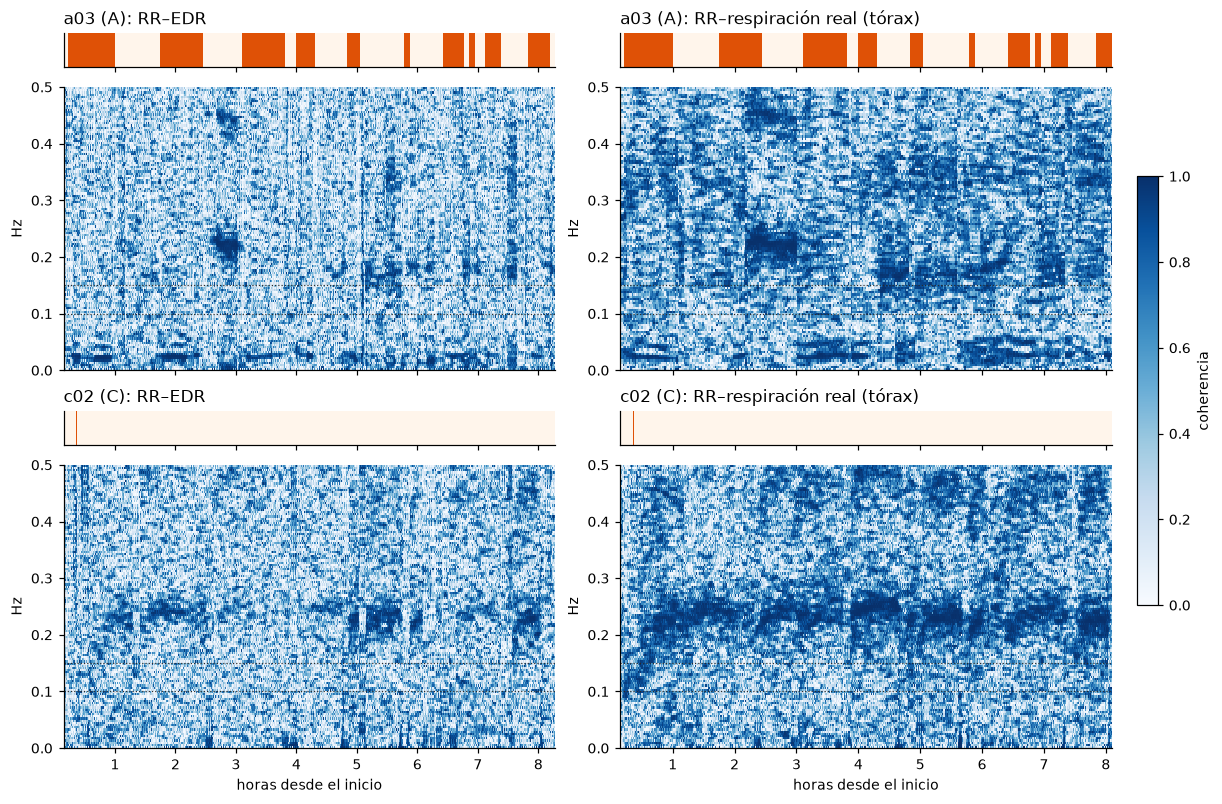
\includegraphics[width=0.85\linewidth]{imagena03.png}
  \caption{Mapas nocturnos de coherencia del registro a03
  (categoría A) y c02 (control). Se compara la serie RR
  con el EDR (izquierda) y con la respiración torácica
  registrada (derecha), utilizando ventanas de 512~s.
  La intensidad del azul representa la coherencia y las
  franjas naranjas superiores indican los minutos
  anotados con apnea. Las líneas punteadas señalan
  0,10 y 0,15~Hz, límites de las bandas evaluadas.}
  \label{fig:mapa}
\end{figure}
\subsection{Estimación honesta en desarrollo}
\label{sec:res-anidada}

Al repetir la elección de la feature, el posprocesamiento y el umbral
mediante validación cruzada anidada por sujetos, F obtuvo un área bajo
la curva media entre grupos de 0,851, con un intervalo de confianza
del 95~\% de 0,760 a 0,916. La sensibilidad fue de 0,839,
la especificidad de 0,748 y el acierto por registro de 0,807.
El área bajo la curva disminuyó 0,024 respecto de la obtenida al
elegir y evaluar el detector con todos los sujetos de desarrollo.

Los cinco grupos eligieron la misma configuración de F: potencia
cruzada RR--EDR con una ventana de 240~s, sin normalización ni
suavizado. Los umbrales variaron entre $-6{,}96$ y $-6{,}91$.
En cambio, la feature de referencia de HRV cambió entre grupos
y obtuvo un área bajo la curva media de 0,729. La diferencia
a favor de F fue de 0,122, con un intervalo de confianza del
95~\% de 0,022 a 0,193. Esta comparación es descriptiva:
la evaluación final de H2 se realiza en test con las
configuraciones fijadas en desarrollo.

Aunque F permitió ordenar las noches según su fracción de apnea,
presentó una sobreestimación de los minutos afectados. El sesgo
fue de $+5{,}0$ minutos de apnea por hora, con límites de acuerdo
de $-21{,}1$ a $+31{,}0$. La categoría A/B/C fue correcta en el
57~\% de las noches y las doce noches de control se clasificaron
como B. Al considerar únicamente la separación entre las noches A
y el resto, el porcentaje de clasificación correcta fue del 83~\%.
Estos resultados muestran que la capacidad de ordenar los registros
no asegura una estimación precisa de la cantidad de apnea
ni de la categoría de cada noche.

\subsection{Evaluación en test}
\label{sec:res-test}

\begin{table}[htbp]
  \centering
  \caption{H2 en test (20 registros, 10 sujetos), corrido una sola vez sobre
           \texttt{congelado-test}. Intervalo al 95~\% con 10\,000 remuestreos de sujetos;
           $p$ bilateral corregido por Holm.}
  \label{tab:test}
  \small
  \begin{tabular}{@{}lcccc@{}}
    \toprule
    Medida & F & Referencia (VLF) & Diferencia (IC 95~\%) & $p$ de Holm \\
    \midrule
    M1: área bajo la curva por minuto & $0{,}785$ & $0{,}793$ & $-0{,}007$ ($-0{,}162$ a $+0{,}112$) & $1{,}00$ \\
    M2: acierto por registro          & $0{,}634$ & $0{,}613$ & $+0{,}021$ ($-0{,}543$ a $+0{,}514$) & $1{,}00$ \\
    \bottomrule
  \end{tabular}
\end{table}

Ninguna de las dos medidas muestra diferencia (Tabla~\ref{tab:test}): H2 no se confirma ni se rechaza con estos datos. Con 10 sujetos los intervalos son muy anchos, así que el resultado tampoco indica que F y la referencia sean equivalentes. Se evaluaron 8.556 de los 9.754 minutos con etiqueta (el 12,3~\% queda afuera, casi todo de c04 y x29, por la regla del 20~\% de RR corregidos). Los resultados secundarios están en la Tabla~\ref{tab:test-sec}.

\begin{table}[htbp]
  \centering
  \caption{Resultados secundarios en test, con los umbrales de desarrollo.}
  \label{tab:test-sec}
  \small
  \begin{tabular}{@{}llcc@{}}
    \toprule
    & Medida & F & Referencia (VLF) \\
    \midrule
    Por minuto & Sensibilidad & $0{,}790$ & $0{,}735$ \\
               & Especificidad & $0{,}642$ & $0{,}686$ \\
               & Exactitud & $0{,}706$ & $0{,}707$ \\
    \midrule
    Por noche  & Sesgo (min de apnea por hora) & $+7{,}3$ & $+5{,}1$ \\
               & Límites de acuerdo & $-27{,}9$ a $+42{,}5$ & $-25{,}4$ a $+35{,}6$ \\
               & Categoría A/B/C correcta & 45~\% & 60~\% \\
               & A contra el resto correcta & 70~\% & 70~\% \\
               & Spearman con el AHI (IC 95~\%) & $0{,}70$ ($0{,}15$ a $0{,}91$) & $0{,}68$ ($-0{,}04$ a $0{,}91$) \\
    \bottomrule
  \end{tabular}
\end{table}

F sobreestima la apnea, como en desarrollo: las 5 noches C quedan como B. \textbf{H1 no se replica}: en los 15 registros A/B de test (8 sujetos), el cociente de coherencias sube con la apnea en solo 4 de 8 sujetos (CPC publicado) y 3 de 8 (esquema v2), con $p$ de Holm 1. Con todos los minutos con etiqueta, ninguna conclusión cambia.

% =====================================================================
\section{Discusión}
\label{sec:discusion}
Los resultados de desarrollo indicaron que la información conjunta
RR--EDR podía aportar a la detección de apnea, pero esa ventaja no se
sostuvo en test. En la validación cruzada anidada, F obtuvo un área
bajo la curva de 0,851 frente a 0,729 de la referencia, mientras que
en test los valores fueron 0,785 y 0,793, respectivamente. Tampoco
se observó una ventaja clara en el acierto por registro. Por lo tanto,
los resultados finales no permiten afirmar que incorporar el EDR
mejore la detección respecto del análisis del RR. Los intervalos
amplios impiden concluir equivalencia, pero la falta de superioridad
no puede atribuirse únicamente al tamaño de la muestra: las
diferencias puntuales en test también fueron pequeñas.

Esta comparación de desarrollo, sin embargo, sobrestimaba la ventaja
de F. En la validación anidada, la referencia se volvía a elegir dentro
de cada grupo y su selección fue inestable: dos de los cinco grupos
obtuvieron un área bajo la curva cercana a 0,53, uno de ellos tras
elegir el cociente entre baja y alta frecuencia, lo que redujo el
promedio a 0,729. La referencia congelada, elegida con todo desarrollo,
alcanzó 0,810 en desarrollo y 0,793 en test, es decir, se mantuvo
estable. Frente a esa referencia, la ventaja de F por minuto ya era
incierta en desarrollo: 0,876 contra 0,810, con una diferencia de
0,066 cuyo intervalo de confianza del 95~\% incluía el cero
($-0{,}004$ a $+0{,}142$). En consecuencia, el cambio entre desarrollo
y test se explica principalmente por la caída de F, de 0,851 en la
validación anidada a 0,785, y no por una mejora de la referencia. La
ventaja más clara de desarrollo estaba en el acierto por registro
(0,81 frente a 0,42), y es también la que menos se reprodujo (0,634
frente a 0,613), en una medida que, con 20 registros y cinco de ellos
casi sin apnea, resulta especialmente variable.

La interpretación de H1 requiere la misma cautela. En desarrollo,
el aumento del cociente de coherencias fue compatible con la
aparición de un acoplamiento lento durante la apnea, sin una
disminución estadísticamente detectable de la coherencia respiratoria.
Sin embargo, esta última observación no demuestra que el acoplamiento
respiratorio se conserve. Además, H1 no se replicó en test: el cambio
tuvo la dirección esperada en solo cuatro de ocho sujetos con las
bandas del CPC publicado. Esto limita la generalización del
comportamiento observado en desarrollo. También debe reconocerse
que la formulación de H1 se modificó después de analizar esos datos:
se pasó de proponer un desplazamiento del acoplamiento hacia
frecuencias menores a plantear la aparición de un componente lento
adicional. La reformulación permite describir mejor lo observado,
pero su respaldo en desarrollo tiene un componente exploratorio
y necesita confirmación independiente.

Por otra parte, el resultado de H1 y la utilidad de F responden
preguntas diferentes. H1 estudia un cociente de coherencias, mientras
que el detector final utiliza potencia cruzada sin ponderarla por
coherencia. Que esta última no mejorara la clasificación indica
que, entre las alternativas evaluadas, su incorporación no aportó
desempeño adicional. No demuestra que la coherencia carezca de
interés fisiológico ni que F mida por sí sola una relación causal
entre respiración y ritmo cardíaco. Al conservar una medida de
potencia sin normalización por noche, también se retienen diferencias
de amplitud entre registros. Estas podrían influir en la aplicación
de un umbral común, aunque este trabajo no permite separar su
contribución de la asociada con la apnea.

La separación por sujetos, la exclusión de grabaciones duplicadas
y el uso de test una sola vez redujeron el riesgo de evaluar el
método sobre información utilizada para elegirlo. No obstante,
la validación anidada tampoco elimina todo el optimismo del
desarrollo. Dentro de cada grupo se repitió la selección de
features, posprocesamiento y umbral, pero algunas decisiones
previas, como la incorporación de la banda de apnea y la regla
de selección, se habían definido observando el conjunto completo.
Además, la regla de empate se reemplazó por una de no inferioridad
después de una primera corrida. Estos cambios fueron documentados,
pero su documentación no elimina la adaptación a los datos.
La estabilidad de F en los cinco grupos muestra consistencia
dentro de desarrollo, sin garantizar su generalización a otros
sujetos. A esto se suma que la identidad de las personas se infirió
a partir de sus perfiles y de la comparación de señales, en lugar
de contar con identificadores confirmados.

Las etapas de preprocesamiento también deben interpretarse según
el alcance de su evaluación. El filtro pasabanda se eligió a partir
de una especificación obtenida sin etiquetas y mantuvo el desempeño
del detector. En cambio, el detector QRS propio y Wiener no
cumplieron el criterio de no inferioridad en el acierto por registro.
Esto justifica no incorporarlos según la regla fijada, pero no
demuestra que sean inferiores ni que carezcan de utilidad para
otros objetivos. El margen de 0,02 fue una tolerancia metodológica,
sin una justificación clínica específica, y su uso en medidas
distintas no supone consecuencias equivalentes. La evaluación
conjunta por minuto y por registro evitó adoptar etapas solo por
una mejora local, aunque también hizo depender su aceptación de
la precisión de ambas estimaciones.

En particular, el detector final conserva las marcas QRS de la
base, por lo que su desempeño no representa todavía el de un
sistema autónomo que recibe únicamente el ECG. La revisión manual
de discrepancias mostró errores tanto del detector propio como
de las marcas de referencia, además de casos dudosos. Por eso,
las métricas de detección de latidos no deben interpretarse como
si la referencia fuera perfecta. Del mismo modo, la mejora del
refinamiento parabólico en la prueba de dos fases respalda una
menor sensibilidad a la posición de muestreo, pero no establece
el error absoluto del pico R frente a una referencia independiente
de mayor frecuencia de muestreo.

La ventana de 240~s permitió estimar las componentes lentas de
interés, a costa de una menor resolución temporal. Aunque se
produce una decisión por minuto, cada valor de F incorpora
información de minutos vecinos. En desarrollo, el 27~\% de los
falsos positivos se ubicó a uno o dos minutos de una apnea;
al excluir los bordes de los episodios, la especificidad aumentó
de 0,748 a 0,796. Esto es compatible con un efecto de mezcla
temporal, pero no explica todos los errores. Los falsos negativos
se concentraron principalmente en el interior de episodios largos
y en pocos sujetos, lo que sugiere que el umbral común no representa
de igual manera a todas las personas. Además, la ventana centrada
y el filtrado ida y vuelta utilizan muestras futuras: la
implementación evaluada corresponde a un análisis fuera de línea
y requeriría modificaciones para funcionar en tiempo real.

El tratamiento de la calidad constituye otra limitación.
Los límites de corrección del RR y la exclusión de minutos con
más del 20~\% de intervalos corregidos no se justificaron mediante
una evaluación específica de esas tolerancias. En test quedó
afuera el 12,3~\% de los minutos con etiqueta, concentrado
principalmente en dos registros. En consecuencia, el desempeño
principal describe los minutos que cumplen las condiciones de
evaluación y no toda la grabación. El análisis con todos los
minutos no modificó las conclusiones, aunque completar decisiones
inválidas con la del minuto válido más cercano no demuestra que
el detector funcione correctamente en esos segmentos. En
desarrollo también se observó una alta tasa de falsos positivos
cuando la ventana contenía señal perdida. Aunque estos casos
representaron una fracción pequeña del total, muestran que la
interpolación puede introducir variaciones lentas que se confundan
con la información buscada.

La elección del umbral de Youden favoreció un equilibrio entre
sensibilidad y especificidad, pero no garantizó una estimación
precisa de la cantidad de apnea por noche. En test, F alcanzó
una sensibilidad de 0,790 y una especificidad de 0,642, con un
sesgo de $+7{,}3$ minutos de apnea por hora y límites de acuerdo
amplios. Las cinco noches de control se clasificaron como B.
Esto muestra por qué una correlación positiva entre las fracciones
estimadas y anotadas no equivale a concordancia: el detector puede
ordenar razonablemente los registros y sobreestimar sus valores.
La clasificación A contra el resto simplificó el resultado, pero
fue incorporada después de observar los problemas de la matriz
A/B/C en desarrollo y debe mantenerse como análisis secundario.
Tampoco la correlación con el AHI permite afirmar que se estime
la gravedad clínica, ya que el detector cuenta minutos afectados,
mientras que el AHI cuenta eventos por hora de sueño.

Los resultados publicados por \textcite{penzel2002} y
\textcite{dechazal2003}, con exactitudes por minuto superiores al
90~\%, muestran que existe información útil para detectar apnea
en el ECG. Sin embargo, no constituyen una comparación directa
con este trabajo, porque difieren los clasificadores, las
particiones y las condiciones de evaluación. La propuesta basada
en una feature y un umbral facilita describir la decisión, pero
esa simplicidad no asegura una mejor generalización. En este
caso, su aporte principal fue permitir analizar de manera
explícita qué información se conserva y dónde falla el criterio. Una continuación debería abordar cada limitación con datos nuevos o una evaluación separada: evaluar F en una cohorte independiente con más sujetos, para tener potencia suficiente; estudiar la estabilidad del umbral entre personas y una calibración por noche que corrija la sobreestimación; justificar con datos las reglas de calidad del RR; corregir en el detector QRS propio la confusión con ondas T empinadas y su arranque sobre tramos con artefacto, para poder prescindir de las marcas de la base; y adaptar la ventana y el filtrado a un esquema causal si se busca un uso en tiempo real.

% =====================================================================
\section{Conclusiones}
\label{sec:conclusiones}

H1 se sostuvo en desarrollo: durante la apnea aumentó la coherencia lenta entre RR y EDR en 11 de 14 sujetos, sin una disminución detectable de la respiratoria, pero no se replicó en test (4 de 8 sujetos). H2 no se confirmó: en test, F obtuvo un área bajo la curva de 0,785 frente a 0,793 de la referencia y un acierto por registro de 0,634 frente a 0,613, sin diferencias significativas. De los temas obligatorios, el detector final conserva el filtro pasabanda diseñado a partir de los datos, el refinamiento del pico R, la segmentación en ventanas de 240~s y la potencia espectral con Lomb como referencia; el detector QRS propio y el filtro de Wiener se evaluaron y no se incorporaron por no cumplir la no inferioridad en el acierto por registro. La principal limitación es el tamaño de test: con 10 sujetos los intervalos son demasiado amplios para afirmar superioridad o equivalencia. Para resolverlo, el paso siguiente es evaluar el criterio en una cohorte independiente y más grande, con un detector de latidos propio y reglas de calidad justificadas con datos.

\label{fin-cuerpo}

% =====================================================================
\printbibliography[heading=bibintoc, title={Referencias}]

% =====================================================================
\clearpage
\appendix
\label{inicio-anexo}

\section{Detalles de métodos y resultados}
\label{anx:detalles}

\subsection*{Revisión manual de las discrepancias del detector propio}

Se sortearon 50 discrepancias entre el detector propio y las marcas de la base (semilla 2026, antes de mirarlas) y se clasificaron viendo 10~s de ECG alrededor de cada una (\texttt{docs/revision\_qrs\_50.csv}). La muestra está dominada por x17 (14 de 50), porque se sorteó sobre todas las discrepancias.

\begin{table}[htbp]
  \centering
  \caption{Clasificación de las 50 discrepancias revisadas.}
  \label{tab:revision}
  \small
  \begin{tabularx}{\textwidth}{@{}lcX@{}}
    \toprule
    Clase & Casos & Patrón principal \\
    \midrule
    Error del detector & 21 & Detección adicional al final de una onda T empinada (x17, x12); oscilaciones rápidas al inicio del registro (c01, x04, c09). \\
    Error de las marcas de la base & 18 & QRS claros sin marca, a menudo negativos o bifásicos. \\
    Dudoso & 11 & Artefacto o ruido que impide decidir. \\
    \bottomrule
  \end{tabularx}
\end{table}

Sin los dudosos, el detector explica 21 de 39 discrepancias: una diferencia con las marcas de la base no es necesariamente un error del detector.

\end{document}
